% Template for PLoS
% Version 3.5 March 2018
%
% % % % % % % % % % % % % % % % % % % % % %
%
% -- IMPORTANT NOTE
%
% This template contains comments intended 
% to minimize problems and delays during our production 
% process. Please follow the template instructions
% whenever possible.
%
% % % % % % % % % % % % % % % % % % % % % % % 
%
% Once your paper is accepted for publication, 
% PLEASE REMOVE ALL TRACKED CHANGES in this file 
% and leave only the final text of your manuscript. 
% PLOS recommends the use of latexdiff to track changes during review, as this will help to maintain a clean tex file.
% Visit https://www.ctan.org/pkg/latexdiff?lang=en for info or contact us at latex@plos.org.
%
%
% There are no restrictions on package use within the LaTeX files except that 
% no packages listed in the template may be deleted.
%
% Please do not include colors or graphics in the text.
%
% The manuscript LaTeX source should be contained within a single file (do not use \input, \externaldocument, or similar commands).
%
% % % % % % % % % % % % % % % % % % % % % % %
%
% -- FIGURES AND TABLES
%
% Please include tables/figure captions directly after the paragraph where they are first cited in the text.
%
% DO NOT INCLUDE GRAPHICS IN YOUR MANUSCRIPT
% - Figures should be uploaded separately from your manuscript file. 
% - Figures generated using LaTeX should be extracted and removed from the PDF before submission. 
% - Figures containing multiple panels/subfigures must be combined into one image file before submission.
% For figure citations, please use "Fig" instead of "Figure".
% See http://journals.plos.org/plosone/s/figures for PLOS figure guidelines.
%
% Tables should be cell-based and may not contain:
% - spacing/line breaks within cells to alter layout or alignment
% - do not nest tabular environments (no tabular environments within tabular environments)
% - no graphics or colored text (cell background color/shading OK)
% See http://journals.plos.org/plosone/s/tables for table guidelines.
%
% For tables that exceed the width of the text column, use the adjustwidth environment as illustrated in the example table in text below.
%
% % % % % % % % % % % % % % % % % % % % % % % %
%
% -- EQUATIONS, MATH SYMBOLS, SUBSCRIPTS, AND SUPERSCRIPTS
%
% IMPORTANT
% Below are a few tips to help format your equations and other special characters according to our specifications. For more tips to help reduce the possibility of formatting errors during conversion, please see our LaTeX guidelines at http://journals.plos.org/plosone/s/latex
%
% For inline equations, please be sure to include all portions of an equation in the math environment.  For example, x$^2$ is incorrect; this should be formatted as $x^2$ (or $\mathrm{x}^2$ if the romanized font is desired).
%
% Do not include text that is not math in the math environment. For example, CO2 should be written as CO\textsubscript{2} instead of CO$_2$.
%
% Please add line breaks to long display equations when possible in order to fit size of the column. 
%
% For inline equations, please do not include punctuation (commas, etc) within the math environment unless this is part of the equation.
%
% When adding superscript or subscripts outside of brackets/braces, please group using {}.  For example, change "[U(D,E,\gamma)]^2" to "{[U(D,E,\gamma)]}^2". 
%
% Do not use \cal for caligraphic font.  Instead, use \mathcal{}
%
% % % % % % % % % % % % % % % % % % % % % % % % 
%
% Please contact latex@plos.org with any questions.
%
% % % % % % % % % % % % % % % % % % % % % % % %

\documentclass[10pt,letterpaper]{article}
\usepackage[top=0.85in,left=2.75in,footskip=0.75in]{geometry}

\usepackage{natbib} % bibliography

\usepackage{tikz}
\usepackage{bm}
\usetikzlibrary{bayesnet}

\usepackage[breakable]{tcolorbox} % for text box

\newtcolorbox[auto counter,width=\textwidth, colback=gray!10, boxrule=0pt]{mybox}[2][]{%
    title=Box~\thetcbcounter: #2, #1}


\usepackage{alltt}

% amsmath and amssymb packages, useful for mathematical formulas and symbols
\usepackage{amsmath,amssymb}

% Use adjustwidth environment to exceed column width (see example table in text)
\usepackage{changepage}

% Use Unicode characters when possible
\usepackage[utf8x]{inputenc}

% textcomp package and marvosym package for additional characters
\usepackage{textcomp,marvosym}

% cite package, to clean up citations in the main text. Do not remove.
\usepackage{cite}

% Use nameref to cite supporting information files (see Supporting Information section for more info)
\usepackage{nameref,hyperref}

% line numbers
\usepackage[right]{lineno}

% ligatures disabled
\usepackage{microtype}
\DisableLigatures[f]{encoding = *, family = * }

% color can be used to apply background shading to table cells only
\usepackage[table]{xcolor}

% array package and thick rules for tables
\usepackage{array}

% create "+" rule type for thick vertical lines
\newcolumntype{+}{!{\vrule width 2pt}}

% create \thickcline for thick horizontal lines of variable length
\newlength\savedwidth
\newcommand\thickcline[1]{%
  \noalign{\global\savedwidth\arrayrulewidth\global\arrayrulewidth 2pt}%
  \cline{#1}%
  \noalign{\vskip\arrayrulewidth}%
  \noalign{\global\arrayrulewidth\savedwidth}%
}

% \thickhline command for thick horizontal lines that span the table
\newcommand\thickhline{\noalign{\global\savedwidth\arrayrulewidth\global\arrayrulewidth 2pt}%
\hline
\noalign{\global\arrayrulewidth\savedwidth}}


% Remove comment for double spacing
%\usepackage{setspace} 
%\doublespacing

% Text layout
\raggedright
\setlength{\parindent}{0.5cm}
\textwidth 5.25in 
\textheight 8.75in

% Bold the 'Figure #' in the caption and separate it from the title/caption with a period
% Captions will be left justified
\usepackage[aboveskip=1pt,labelfont=bf,labelsep=period,justification=raggedright,singlelinecheck=off]{caption}
\renewcommand{\figurename}{Fig}

% Use the PLoS provided BiBTeX style
\bibliographystyle{plos2015}

% Remove brackets from numbering in List of References
\makeatletter
\renewcommand{\@biblabel}[1]{\quad#1.}
\makeatother



% Header and Footer with logo
\usepackage{lastpage,fancyhdr,graphicx}
\usepackage{epstopdf}
%\pagestyle{myheadings}
\pagestyle{fancy}
\fancyhf{}
%\setlength{\headheight}{27.023pt}
%\lhead{\includegraphics[width=2.0in]{PLOS-submission.eps}}
\rfoot{\thepage/\pageref{LastPage}}
\renewcommand{\headrulewidth}{0pt}
\renewcommand{\footrule}{\hrule height 2pt \vspace{2mm}}
\fancyheadoffset[L]{2.25in}
\fancyfootoffset[L]{2.25in}
\lfoot{\today}

%% Include all macros below

\newcommand{\lorem}{{\bf LOREM}}
\newcommand{\ipsum}{{\bf IPSUM}}

%% END MACROS SECTION


\begin{document}
\vspace*{0.2in}

% Title must be 250 characters or less.
\begin{flushleft}
{\Large
\textbf\newline{LinguaPhylo: a probabilistic model specification language for
  reproducible phylogenetic analyses} % Please use "sentence case" for title and headings (capitalize only the first word in a title (or heading), the first word in a subtitle (or subheading), and any proper nouns).
}
\newline
% Insert author names, affiliations and corresponding author email (do not include titles, positions, or degrees).
\\
Alexei J. Drummond\textsuperscript{1,2}*,
Dong Xie\textsuperscript{1},
Fabio K Mendes\textsuperscript{1,2}
\\
\bigskip
\textbf{1} School of Biological Sciences, University of Auckland, Auckland, New Zealand
\\
\textbf{2} School of Computer Science, University of Auckland, Auckland, New Zealand
\\
\bigskip

% Insert additional author notes using the symbols described below. Insert symbol callouts after author names as necessary.
% 
% Remove or comment out the author notes below if they aren't used.
%
% Primary Equal Contribution Note

% Use the asterisk to denote corresponding authorship and provide email address in note below.
* a.drummond@auckland.ac.nz

\end{flushleft}
% Please keep the abstract below 300 words
\section*{Abstract}
  Phylogenetic models have become increasingly complex and the data sets addressed larger and more rich.
  Yet there is no succinct language to accurately specify the details of a phylogenetic model for the purposes of reproducibility or reuse.
  We present a new language to specify the details of a phylogenetic model that is both human and machine readable.
  We also report on the development of a graphical software package that can be used to construct and simulate data from
  models in this new language, as well as create natural language narratives that can form the basis of a description of the model for the method section of a manuscript.
  Finally we report on a command-line program that can be used to generate XML for the BEAST2 software package based
  on a model specified in this new language.
  These tools together should aid in the goal of reproducibility and reuse of probabilistic phylogenetic models.


% Please keep the Author Summary between 150 and 200 words
% Use first person. PLOS ONE authors please skip this step. 
% Author Summary not valid for PLOS ONE submissions.   
\section*{Author summary}
  We describe a succinct domain-specific language to accurately specify the details of a phylogenetic model for the purposes of reproducibility or reuse.
  In addition we have developed a graphical software package that can be used to construct and simulate data from models described in this new language, as well as create natural language narratives that can form the basis of a description of the model for the method section of a manuscript.
  Finally we report on a command-line program that can be used to generate XML for the BEAST2 software package based on a model specified in this new language.
  These tools together should aid in the goal of reproducibility and reuse of probabilistic phylogenetic models.


\linenumbers

% Use "Eq" instead of "Equation" for equation citations.
\section*{Introduction}

Transparency is a scientific ideal, and replicability and
reproducibility lie at the heart of the scientific endeavor
\citep{nas19,munafo17}.
Despite this being a non-contentious point, only recently have
systematic examinations of the literature begun to reveal that
reproducibility is largely overlooked in pratice.
Metaresearch efforts have uncovered the so-called ``reproducibility
crisis'' \citep{baker16} in many disciplines (but see
\citep{fanneli18}), among which the dimension of the problem varies.
In psychology, for example, a larger scale replication attempt was
successful in only 39\% of surveyed studies \citep{openscience15},
with numbers being less discouraging in other attempts (62\%;
\citep{camerer18}), and in other domains (e.g., economics, 61.1\%,
\citep{camerer16}; cancer biology, X\%, [citation]).

* In evolutionary biology we don't know very well yet, but some
initial papers show it also happens.

* Phylogenetics in particular is now highly computational, and the
intersection with computer science puts this area of evolutionary
biology in a special position to address reproducibility.

A new paradigm for scientific computing and data science has begun to
emerged in the last decade.
A recent example is the publication of the
first ``computationally reproducible article'' using eLife's
Reproducible Document Stack which blends features of a traditional
manuscript with live code, data and interactive figures.

Although standard tools for statistical phylogenetics provide a degree
of reproducibility and reusability through popular open-source
software and computer-readable data file formats, there is still much
to do.
The ability to construct and accurately communicate
probabilistic models in phylogenetics is frustratingly
underdeveloped.
There is low interoperability between different
inference packages (e.g. BEAST1, BEAST2, MrBayes, RevBayes), and the
file formats that these software use have low readability for
researchers.

In this paper we describe two related projects, LinguaPhylo (LPhy for
short) and LPhyBEAST.

\section*{Design and Implementation}

\subsection*{A concise domain-specific language for phylogenetic inference}

LinguaPhylo is a model specification language to concisely and
precisely define probabilistic phylogenetic models.
The aim is to work
towards a common language for probabilistic models of phylogenetic
evolution.
This language should be readable by both humans and
computers.
Box \ref{box1} shows a simple example.

\begin{mybox}[label=box1]{A simple phylogenetic model}
 % \begin{minipage}[t]{0.60\textwidth}
 
 \begin{enumerate}
 \item Modeling language
    {\singlespacing
\begin{alltt}
model \{
  \textcolor{green}{\(\lambda\)} ~ \textcolor{blue}{LogNormal}(\textcolor{gray}{meanlog=}\textcolor{magenta}{3.0}, \textcolor{gray}{sdlog=}\textcolor{magenta}{1.0});
  \textcolor{green}{\(\psi\)} ~ \textcolor{blue}{Yule}(\textcolor{gray}{lambda=}\textcolor{green}{\(\lambda\)}, \textcolor{gray}{n=}\textcolor{magenta}{16});
  \textcolor{green}{D} ~ \textcolor{blue}{PhyloCTMC}(\textcolor{gray}{L=}\textcolor{magenta}{200}, \textcolor{gray}{Q=}\textcolor{magenta!80!black}{jukesCantor}(), \textcolor{gray}{tree=}\textcolor{green}{\(\psi\)});
\}
\end{alltt}
}
%  \end{minipage}%
%\begin{minipage}[t]{0.40\textwidth}
\item Graphical model
\\\\
{\centering
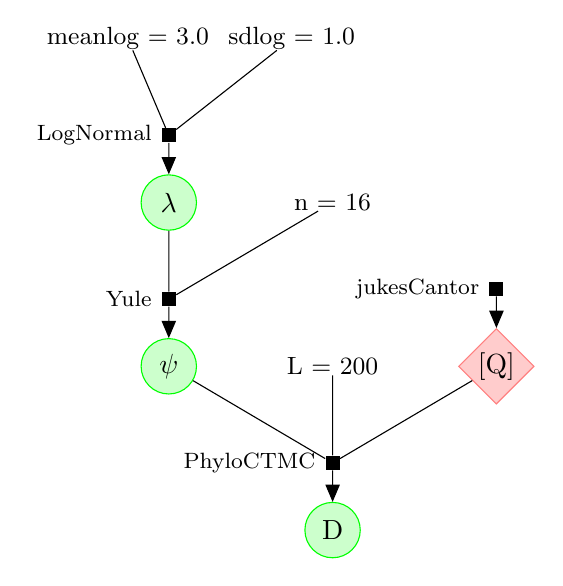
\begin{tikzpicture}[scale=0.52,
dstyle/.style={draw=blue!50,fill=blue!20},
vstyle/.style={draw=green,fill=green!20},
cstyle/.style={font=\small},
detstyle/.style={draw=red!50,fill=red!20}
]
\node[const, cstyle] at (1.0, -0.0) (602717583) {meanlog = 3.0};
\node[const, cstyle] at (5.0, -0.0) (897996787) {sdlog = 1.0};
\node[latent, vstyle] at (2.0, -4.0) (lambda) {$\lambda$};
\node[const, cstyle] at (6.0, -4.0) (2011155364) {n = 16};
\node[latent, vstyle] at (2.0, -8.0) (psi) {$\psi$};
\node[const, cstyle] at (6.0, -8.0) (1992433642) {L = 200};
\node[det, detstyle] at (10.0, -8.0) (258223775) {[Q]};
\node[latent, vstyle] at (6.0, -12.0) (D) {D};
\factor[above=of lambda] {LogNormallambda} {left:LogNormal} {} {} ; %
\factoredge {602717583, 897996787} {LogNormallambda} {lambda}; %
\factor[above=of psi] {Yulepsi} {left:Yule} {} {} ; %
\factoredge {lambda, 2011155364} {Yulepsi} {psi}; %
\factor[above=of 258223775] {jukesCantor258223775} {left:jukesCantor} {} {} ; %
\factoredge {} {jukesCantor258223775} {258223775}; %
\factor[above=of D] {PhyloCTMCD} {left:PhyloCTMC} {} {} ; %
\factoredge {1992433642, 258223775, psi} {PhyloCTMCD} {D}; %
\end{tikzpicture}}
%\end{minipage}

\item Posterior

$$P(\psi, \lambda | D) \propto P(D | \psi) P(\psi | \lambda) P(\lambda) $$

\end{enumerate}

\end{tcolorbox}

Each of the lines in this model specification expresses how a random
variable (to the left of the tilde) is generated by a generative
distribution to the right.

The first line creates a random variable (\texttt{lambda}), that is
log-normally distributed.
The second line creates a tree (\texttt{tree}) with 16 taxa from the
Yule process with a lineage birth rate equal to \texttt{lambda}.
The third line produces a multiple sequence alignment (\texttt{D})
with a length of 200, by simulating a Jukes Cantor model of sequence
evolution down the branches of  \texttt{tree}.
As you can see, each of the random variables depends on the previous,
so this is a hierarchical model that ultimately defines a probability
distribution over sequence alignments of size $16 \times 200$.

To construct an analysis of a data set with this model we add a data block:

{\small
\begin{alltt}
data \{
  D = \textcolor{magenta!80!black}{readNexus}(\textcolor{gray}{file=}\textcolor{magenta}{"data/primate.nex"});
  L = D.\textcolor{magenta!80!black}{nchar}();
  taxa = D.\textcolor{magenta!80!black}{taxa}();
\}
model \{
  \textcolor{green}{lambda} ~ \textcolor{blue}{LogNormal}(\textcolor{gray}{meanlog=}\textcolor{magenta}{3.0}, \textcolor{gray}{sdlog=}\textcolor{magenta}{1.0});
  \textcolor{green}{tree} ~ \textcolor{blue}{Yule}(\textcolor{gray}{lambda=}\textcolor{green}{lambda}, \textcolor{gray}{taxa=}taxa);
  \textcolor{green}{D} ~ \textcolor{blue}{PhyloCTMC}(\textcolor{gray}{L=}L, \textcolor{gray}{Q=}\textcolor{magenta!80!black}{jukesCantor}(), \textcolor{gray}{tree=}\textcolor{green}{tree});
\}
\end{alltt}}

These two blocks of statements contain all the information needed to define
a Bayesian phylogenetic analysis of a multiple sequence alignment.
The data block may contain literals, and deterministic values, including those read in from a file, but not random variables or generative distributions.
The model block contains all random variables, generative distributions and boundary conditions that define the model.
If a value in the data block has the same name as a random variable in the model block, then that signifies that the data block value is an observation of the random variable with the same name.


So by assigning the alignment in file
``data/primate.nex'' to the name D in the data block we are saying that the random variable in the model named D has
been observed, and we will infer all the other random variables
(tree and lambda in this example) in the model from that observed sequence alignment.

% Results and Discussion can be combined.
\section*{Results}
Nulla mi mi, venenatis sed ipsum varius, Table~\ref{table1} volutpat euismod diam. Proin rutrum vel massa non gravida. Quisque tempor sem et dignissim rutrum. Lorem ipsum dolor sit amet, consectetur adipiscing elit. Morbi at justo vitae nulla elementum commodo eu id massa. In vitae diam ac augue semper tincidunt eu ut eros. Fusce fringilla erat porttitor lectus cursus, vel sagittis arcu lobortis. Aliquam in enim semper, aliquam massa id, cursus neque. Praesent faucibus semper libero.

% Place tables after the first paragraph in which they are cited.
\begin{table}[!ht]
\begin{adjustwidth}{-2.25in}{0in} % Comment out/remove adjustwidth environment if table fits in text column.
\centering
\caption{
{\bf Table caption Nulla mi mi, venenatis sed ipsum varius, volutpat euismod diam.}}
\begin{tabular}{|l+l|l|l|l|l|l|l|}
\hline
\multicolumn{4}{|l|}{\bf Heading1} & \multicolumn{4}{|l|}{\bf Heading2}\\ \thickhline
$cell1 row1$ & cell2 row 1 & cell3 row 1 & cell4 row 1 & cell5 row 1 & cell6 row 1 & cell7 row 1 & cell8 row 1\\ \hline
$cell1 row2$ & cell2 row 2 & cell3 row 2 & cell4 row 2 & cell5 row 2 & cell6 row 2 & cell7 row 2 & cell8 row 2\\ \hline
$cell1 row3$ & cell2 row 3 & cell3 row 3 & cell4 row 3 & cell5 row 3 & cell6 row 3 & cell7 row 3 & cell8 row 3\\ \hline
\end{tabular}
\begin{flushleft} Table notes Phasellus venenatis, tortor nec vestibulum mattis, massa tortor interdum felis, nec pellentesque metus tortor nec nisl. Ut ornare mauris tellus, vel dapibus arcu suscipit sed.
\end{flushleft}
\label{table1}
\end{adjustwidth}
\end{table}


%PLOS does not support heading levels beyond the 3rd (no 4th level headings).
\subsection*{\lorem\ and \ipsum\ nunc blandit a tortor}
\subsubsection*{3rd level heading} 
Maecenas convallis mauris sit amet sem ultrices gravida. Etiam eget sapien nibh. Sed ac ipsum eget enim egestas ullamcorper nec euismod ligula. Curabitur fringilla pulvinar lectus consectetur pellentesque. Quisque augue sem, tincidunt sit amet feugiat eget, ullamcorper sed velit. Sed non aliquet felis. Lorem ipsum dolor sit amet, consectetur adipiscing elit. Mauris commodo justo ac dui pretium imperdiet. Sed suscipit iaculis mi at feugiat. 

\begin{enumerate}
	\item{react}
	\item{diffuse free particles}
	\item{increment time by dt and go to 1}
\end{enumerate}


\subsection*{Sed ac quam id nisi malesuada congue}

Nulla mi mi, venenatis sed ipsum varius, volutpat euismod diam. Proin rutrum vel massa non gravida. Quisque tempor sem et dignissim rutrum. Lorem ipsum dolor sit amet, consectetur adipiscing elit. Morbi at justo vitae nulla elementum commodo eu id massa. In vitae diam ac augue semper tincidunt eu ut eros. Fusce fringilla erat porttitor lectus cursus, vel sagittis arcu lobortis. Aliquam in enim semper, aliquam massa id, cursus neque. Praesent faucibus semper libero.

\begin{itemize}
	\item First bulleted item.
	\item Second bulleted item.
	\item Third bulleted item.
\end{itemize}

\section*{Discussion}
Nulla mi mi, venenatis sed ipsum varius, Table~\ref{table1} volutpat euismod diam. Proin rutrum vel massa non gravida. Quisque tempor sem et dignissim rutrum. Lorem ipsum dolor sit amet, consectetur adipiscing elit. Morbi at justo vitae nulla elementum commodo eu id massa. In vitae diam ac augue semper tincidunt eu ut eros. Fusce fringilla erat porttitor lectus cursus, vel sagittis arcu lobortis. Aliquam in enim semper, aliquam massa id, cursus neque. Praesent faucibus semper libero~\cite{bib3}.

\section*{Conclusion}

CO\textsubscript{2} Maecenas convallis mauris sit amet sem ultrices gravida. Etiam eget sapien nibh. Sed ac ipsum eget enim egestas ullamcorper nec euismod ligula. Curabitur fringilla pulvinar lectus consectetur pellentesque. Quisque augue sem, tincidunt sit amet feugiat eget, ullamcorper sed velit. 

Sed non aliquet felis. Lorem ipsum dolor sit amet, consectetur adipiscing elit. Mauris commodo justo ac dui pretium imperdiet. Sed suscipit iaculis mi at feugiat. Ut neque ipsum, luctus id lacus ut, laoreet scelerisque urna. Phasellus venenatis, tortor nec vestibulum mattis, massa tortor interdum felis, nec pellentesque metus tortor nec nisl. Ut ornare mauris tellus, vel dapibus arcu suscipit sed. Nam condimentum sem eget mollis euismod. Nullam dui urna, gravida venenatis dui et, tincidunt sodales ex. Nunc est dui, sodales sed mauris nec, auctor sagittis leo. Aliquam tincidunt, ex in facilisis elementum, libero lectus luctus est, non vulputate nisl augue at dolor. For more information, see \nameref{S1_Appendix}.

\section*{Supporting information}

% Include only the SI item label in the paragraph heading. Use the \nameref{label} command to cite SI items in the text.
\paragraph*{S1 Fig.}
\label{S1_Fig}
{\bf Bold the title sentence.} Add descriptive text after the title of the item (optional).

\paragraph*{S2 Fig.}
\label{S2_Fig}
{\bf Lorem ipsum.} Maecenas convallis mauris sit amet sem ultrices gravida. Etiam eget sapien nibh. Sed ac ipsum eget enim egestas ullamcorper nec euismod ligula. Curabitur fringilla pulvinar lectus consectetur pellentesque.

\paragraph*{S1 File.}
\label{S1_File}
{\bf Lorem ipsum.}  Maecenas convallis mauris sit amet sem ultrices gravida. Etiam eget sapien nibh. Sed ac ipsum eget enim egestas ullamcorper nec euismod ligula. Curabitur fringilla pulvinar lectus consectetur pellentesque.

\paragraph*{S1 Video.}
\label{S1_Video}
{\bf Lorem ipsum.}  Maecenas convallis mauris sit amet sem ultrices gravida. Etiam eget sapien nibh. Sed ac ipsum eget enim egestas ullamcorper nec euismod ligula. Curabitur fringilla pulvinar lectus consectetur pellentesque.

\paragraph*{S1 Appendix.}
\label{S1_Appendix}
{\bf Lorem ipsum.} Maecenas convallis mauris sit amet sem ultrices gravida. Etiam eget sapien nibh. Sed ac ipsum eget enim egestas ullamcorper nec euismod ligula. Curabitur fringilla pulvinar lectus consectetur pellentesque.

\paragraph*{S1 Table.}
\label{S1_Table}
{\bf Lorem ipsum.} Maecenas convallis mauris sit amet sem ultrices gravida. Etiam eget sapien nibh. Sed ac ipsum eget enim egestas ullamcorper nec euismod ligula. Curabitur fringilla pulvinar lectus consectetur pellentesque.

\section*{Acknowledgments}
Cras egestas velit mauris, eu mollis turpis pellentesque sit amet. Interdum et malesuada fames ac ante ipsum primis in faucibus. Nam id pretium nisi. Sed ac quam id nisi malesuada congue. Sed interdum aliquet augue, at pellentesque quam rhoncus vitae.

\nolinenumbers

% Either type in your references using
% \begin{thebibliography}{}
% \bibitem{}
% Text
% \end{thebibliography}
%
% or
%
% Compile your BiBTeX database using our plos2015.bst
% style file and paste the contents of your .bbl file
% here. See http://journals.plos.org/plosone/s/latex for 
% step-by-step instructions.
% 
\bibliography{linguaPhylo}



\end{document}

